\documentclass[runningheads]{llncs}
\usepackage[T1]{fontenc}
\usepackage{amsmath,amssymb}
\usepackage{booktabs}
\usepackage{graphicx}
\usepackage{xcolor}
\usepackage[colorlinks=true,linkcolor=blue!50!black,citecolor=blue!50!black,urlcolor=blue!50!black]{hyperref}
\renewcommand\UrlFont{\color{blue!50!black}\rmfamily}
\newcommand{\nDev}{328}
\newcommand{\nTest}{768}
\newcommand{\nTasks}{1096}
\newcommand{\tunedSim}{0.8}
\newcommand{\tunedTrust}{0.0}
\newcommand{\tunedEv}{0.1}
\newcommand{\tunedStale}{0.05}
\newcommand{\tunedHL}{365}
\newcommand{\devMRR}{0.693}
\newcommand{\devHit}{0.823}
\newcommand{\gridSize}{420}
\newcommand{\hitFiveSnap}{0.641}
\newcommand{\hitOneSnap}{0.378}
\newcommand{\mrrSnap}{0.497}
\newcommand{\hitFiveEmv}{0.684}
\newcommand{\hitOneEmv}{0.406}
\newcommand{\mrrEmv}{0.532}
\newcommand{\hitFiveTuned}{0.751}
\newcommand{\hitOneTuned}{0.454}
\newcommand{\mrrTuned}{0.585}
\newcommand{\hitFivePlain}{0.551}
\newcommand{\hitOnePlain}{0.333}
\newcommand{\mrrPlain}{0.433}
\newcommand{\hitFiveNaive}{0.612}
\newcommand{\hitOneNaive}{0.357}
\newcommand{\mrrNaive}{0.470}
\newcommand{\hitFivePop}{0.451}
\newcommand{\hitOnePop}{0.083}
\newcommand{\mrrPop}{0.244}
\newcommand{\hitFiveRec}{0.451}
\newcommand{\hitOneRec}{0.189}
\newcommand{\mrrRec}{0.307}
\newcommand{\deadPlain}{0.179}
\newcommand{\deadNaive}{0.181}
\newcommand{\deadBlind}{0.015}
\newcommand{\contamPlain}{0.267}
\newcommand{\deadShare}{20}
\newcommand{\plainDeadTasks}{54}
\newcommand{\shufSnapFive}{0.130}
\newcommand{\shufEmvFive}{0.461}
\newcommand{\leakSnapOne}{0.999}
\newcommand{\leakEmvOne}{0.999}
\newcommand{\trustMean}{1.000}
\newcommand{\trustECE}{0.594}
\newcommand{\aurocGapEmv}{0.751}
\newcommand{\aurocGapSnap}{0.820}
\newcommand{\aurocGapTuned}{0.783}
\newcommand{\aurocTrustEmv}{0.500}
\newcommand{\covTwentyEmv}{0.3}
\newcommand{\accTwentyEmv}{100.0}
\newcommand{\covTwentyTuned}{5.1}
\newcommand{\accTwentyTuned}{97.4}
\newcommand{\covTwentySnap}{6.2}
\newcommand{\accTwentySnap}{93.8}
\newcommand{\covTenEmv}{5.7}
\newcommand{\accTenEmv}{93.2}
\newcommand{\covTenTuned}{14.3}
\newcommand{\accTenTuned}{92.7}
\newcommand{\covTenSnap}{16.7}
\newcommand{\accTenSnap}{88.3}
\newcommand{\covFiveEmv}{15.9}
\newcommand{\accFiveEmv}{86.1}
\newcommand{\covFiveTuned}{29.6}
\newcommand{\accFiveTuned}{82.8}
\newcommand{\covFiveSnap}{31.5}
\newcommand{\accFiveSnap}{74.8}
\newcommand{\dTunedSnapFive}{0.111}
\newcommand{\dTunedSnapLo}{0.082}
\newcommand{\dTunedSnapHi}{0.142}
\newcommand{\tunedOnly}{117}
\newcommand{\snapOnly}{32}
\newcommand{\dEmvSnapFive}{0.043}
\newcommand{\dEmvSnapLo}{0.000}
\newcommand{\dEmvSnapHi}{0.086}
\newcommand{\pEmvSnap}{0.112}
\newcommand{\dEmvPlainFive}{0.133}
\newcommand{\dEmvPlainLo}{0.090}
\newcommand{\dEmvPlainHi}{0.176}
\newcommand{\dTunedEmvFive}{0.068}
\newcommand{\dTunedEmvLo}{0.038}
\newcommand{\dTunedEmvHi}{0.100}
\newcommand{\dTunedSnapOne}{0.077}
\newcommand{\dSnapPlainFive}{0.090}
\newcommand{\ablNoTrust}{+0.021}
\newcommand{\ablNoStale}{+0.035}
\newcommand{\repFastSnap}{0.541}
\newcommand{\repFastEmv}{0.645}
\newcommand{\repFastTuned}{0.715}
\newcommand{\repFastPop}{0.640}
\newcommand{\repFastPlain}{0.384}
\newcommand{\repYtdlpSnap}{0.801}
\newcommand{\repYtdlpEmv}{0.689}
\newcommand{\repYtdlpTuned}{0.893}
\newcommand{\repYtdlpPop}{0.260}
\newcommand{\repYtdlpPlain}{0.796}
\newcommand{\repBuSnap}{0.605}
\newcommand{\repBuEmv}{0.698}
\newcommand{\repBuTuned}{0.698}
\newcommand{\repBuPop}{0.463}
\newcommand{\repBuPlain}{0.502}
\newcommand{\nClaims}{1750}

\renewcommand{\dTunedSnapLo}{0.081}\renewcommand{\dTunedSnapHi}{0.141}
\graphicspath{{figures/}}
\setlength{\emergencystretch}{3em}
\newcommand{\sys}{EmemoVeri}

\begin{document}
\title{Which Parts of Repository Memory Pay Off for Coding Agents? A Leakage-Controlled Component Analysis on Real Git History}
\titlerunning{Which Parts of Repository Memory Pay Off for Coding Agents?}
\author{Mihit}
\authorrunning{Mihit}
\institute{IILM University, Greater Noida, India}
\maketitle

\begin{abstract}
Coding agents that keep memory about a repository must cope with knowledge that goes stale, is contradicted, or was never reliable. We ask which ingredients of such a memory actually help, using \sys{}, a design that attaches typed, timestamped evidence to file-level claims, evolves a claim state, tracks trust, and ranks claims with an evidence-, staleness- and scope-aware score. We replay git history on one chronological clock and ask a memory to rank the files a \emph{future} commit will modify from its subject line, with reference files and claim relations read from git and a leak canary, a shuffled-query control and a dev/test split in time. On three development repositories (\nTest{} test tasks) a cumulative ladder shows that the measurable benefit comes from similarity plus two cheap ingredients, removing deleted files (+0.029 Hit@5) and a change-frequency prior (+0.087); typed evidence adds +0.016 (interval includes zero), trust and staleness add nothing. A dev-tuned \sys{} beats snapshot retrieval by +\dTunedSnapFive{} Hit@5 but is indistinguishable from a tuned similarity+state+recency+popularity baseline. We then freeze all systems and evaluate them, under a protocol fixed beforehand, on twelve repositories never used in design or tuning (4{,}636 tasks): the tuned gain over snapshot retrieval replicates (+0.090 [0.064, 0.117], 12 of 12 repositories), the tuned design is again no better than the simple prior baseline ($-$0.004 [$-$0.008, 0.001]), and the blueprint weights are not reliably better than snapshot retrieval. State tracking removes every stale-path suggestion and carries history across renames (82\% against 23\% without carry-over). Trust saturates (AUROC 0.50) and the abstention rule is no better than a similarity gap. We release code, tests and results, and document eight defects fixed in the original implementation.
\end{abstract}
\keywords{Coding agents \and Agent memory \and Repository mining \and Retrieval \and Evaluation}

\section{Introduction}
A coding agent that works on the same repository over weeks accumulates knowledge: which module owns a behaviour, which API replaced a deprecated one, which test guards an invariant. Such knowledge decays. Files are renamed or deleted, changes are reverted, and conclusions drawn from one commit are overturned by the next. A memory that simply stores and retrieves text treats an outdated statement and a current one alike. \sys{} is a design that tries to address this by tracking \emph{evidence} for each remembered claim and letting the claim's \emph{state} change as evidence arrives.

The design is easy to describe and hard to evaluate honestly. Real tasks require a model in the loop, long runs, and labels that do not depend on the memory under test. Synthetic scenarios are cheap, but when the generator decides which claim is correct by giving it higher trust, fresher timestamps and test evidence, it rewards exactly the features the scorer uses. This was true of the original \sys{} experiments, and we do not use them as evidence here. Rather than asking whether one configuration scores well, we ask \emph{which ingredients of a repository memory pay for themselves, and in which settings}. Eight questions structure the paper: \textbf{RQ1} does temporal memory beat static retrieval; \textbf{RQ2} which components buy the gain; \textbf{RQ3} is the gain just recency and popularity; \textbf{RQ4} do evidence, trust and staleness matter; \textbf{RQ5} does it generalise across repositories and retrieval backends; \textbf{RQ6} does it help when queries are vague; \textbf{RQ7} does the state machine handle lifecycle events such as deletions and renames; \textbf{RQ8} do the answers hold on repositories never used in design or tuning.

\begin{figure}[t]\centering
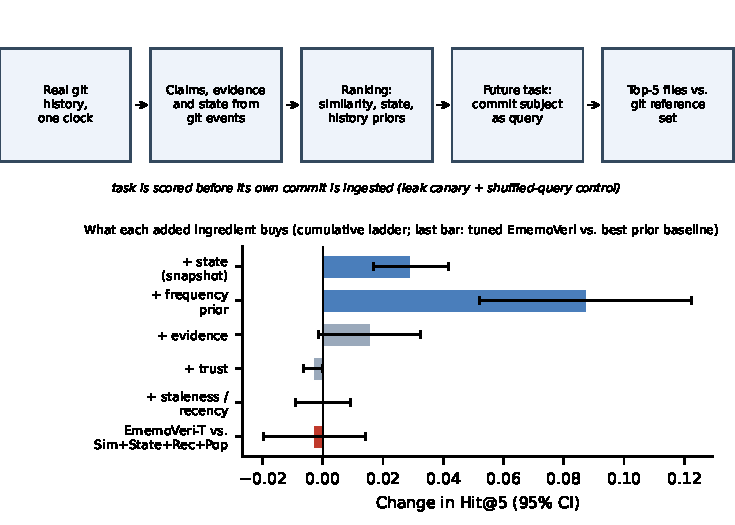
\includegraphics[width=\linewidth]{fig_overview.pdf}
\caption{Overview. Memory is built from git events on one clock and queried with the subject of a future commit. The bars give the measured effect of each added ingredient on Hit@5 (Section~\ref{sec:ladder}); the last bar compares dev-tuned \sys{} with the best tuned history-prior baseline (Section~\ref{sec:prior}).}
\label{fig:overview}
\end{figure}

\noindent The contributions are as follows.
\begin{enumerate}
\item \textbf{A leakage-controlled replay benchmark on real history.} Memory is built commit by commit on a single clock; every task is scored before its own commit is ingested; relations and reference files come from git. A leak canary verifies that the harness detects leakage and a shuffled-query control measures how much of a score is independent of the query (Section~\ref{sec:bench}).
\item \textbf{A component ladder and strong history-prior baselines.} A cumulative ladder from similarity to the full score, and tuned similarity+recency+popularity baselines with and without state, separate what state, frequency, evidence, trust and staleness each contribute (Sections~\ref{sec:ladder}--\ref{sec:prior}).
\item \textbf{A robustness battery.} Three retrieval backends, leave-one-repository-out tuning, query degradation, a staleness sweep, and bootstrap resampling by task, by repository-month block and by file cluster (Sections~\ref{sec:components}--\ref{sec:valid}).
\item \textbf{A lifecycle evaluation and an honest negative result.} Knowing which files still exist and a cheap change-frequency prior account for most of the measured gain, whereas the trust value and the abstention rule add nothing in this evidence regime. Deletions and renames are also evaluated directly as lifecycle events (Section~\ref{sec:life}).
\item \textbf{A pre-declared confirmation on twelve held-out repositories.} All systems are frozen and judged at the repository level on 4{,}636 tasks from repositories that played no part in design, debugging or tuning (Section~\ref{sec:heldout}).
\item \textbf{An audit of the original implementation.} Eight defects, including a leakage guard that leaked, are documented, fixed and covered by regression tests (Section~\ref{sec:audit}).
\end{enumerate}
We do not claim that \sys{} improves end-to-end agent success, and we do not use real issue text: no language model is in the loop and queries are commit subjects. We claim only what the benchmark measures.

\section{Related work}
\textbf{Memory for language-model agents.} Retrieval-augmented generation~\cite{lewis2020rag} conditions a model on retrieved passages. Later agent-memory work adds rules for writing, updating and forgetting. MemGPT pages information between context tiers~\cite{packer2023memgpt}; Generative Agents score memories by recency, importance and relevance~\cite{park2023generative}; Reflexion keeps written self-feedback between attempts~\cite{shinn2023reflexion}; Mem0~\cite{chhikara2025mem0} and A-MEM~\cite{xu2025amem} restructure stored memories as new information arrives. LongMemEval probes long-horizon recall in chat assistants, including how they handle changed facts~\cite{wu2024longmemeval}. The memory studied here describes a code repository instead, its updates are version-control events, and the correct answer can be read from the history itself.

\textbf{Repository-level code assistance.} SWE-bench~\cite{jimenez2024swebench} and SWE-agent~\cite{yang2024sweagent} judge whether an agent resolves real issues, and RepoCoder~\cite{zhang2023repocoder} retrieves repository context repeatedly during code completion. All three need a model in the loop. We instead isolate the memory component and measure only which files it surfaces.

\textbf{Mining software repositories.} Mining co-changes recommends files that tend to change together~\cite{zimmermann2005mining}; recently changed or frequently changed code predicts where faults appear~\cite{kim2007cache,hassan2009complexity}; and information-retrieval bug localisation ranks files against a bug report~\cite{zhou2012buglocator}. Our finding that recency and change frequency are hard to beat agrees with this line of work. Kalliamvakou et al.~\cite{kalliamvakou2014perils} catalogue the hazards of mining GitHub, and we read history directly with \texttt{git}, as tools such as PyDriller~\cite{spadini2018pydriller} do. Selective classification~\cite{geifman2017selective} and expected calibration error~\cite{guo2017calibration} frame our analysis of abstention and trust.

\section{The \sys{} mechanism}
\label{sec:mech}
\textbf{Claims, evidence, state.} A claim has a statement, a scope, a state and a trust value in $[0,1]$. Evidence items have a type (commit, test, issue, documentation, agent observation, external), a relation (corroborates, refines, contradicts, supersedes), a timestamp and a strength. A claim starts PROVISIONAL and moves to CORROBORATED, REFINED or CONTESTED as evidence accumulates. SUPERSEDED is terminal: later evidence is recorded for provenance but cannot revive the claim (Section~\ref{sec:audit}).

\textbf{Trust.} The default update is sequential and clamped, $t \leftarrow \mathrm{clip}(t + \eta\, w_e,0,1)$, $\eta=0.35$. We also implement a pooled clamped update and an order-invariant non-saturating update $t=\sigma(\mathrm{logit}(t_0)+\eta\sum_e w_e)$.

\textbf{Retrieval score.} For a query with scope $q$ at reference time $\tau$,
\begin{equation}
s = 0.45\,\mathrm{sim} + 0.25\,\mathrm{trust} + 0.20\,\mathrm{evid} + 0.10\,\mathrm{scope} - 0.10\,\mathrm{stale},
\end{equation}
where $\mathrm{evid}=E/(E+5)$ for total evidence strength $E$, $\mathrm{stale}=1-2^{-\Delta/H}$ with $\Delta$ the time since the last update and $H=90$ days, and scope is 1 for a same-scope claim. SUPERSEDED claims are excluded, and a local-first policy admits a cross-scope claim only if it beats the best local score by a margin. Note that $-w\,\mathrm{stale}=w\,2^{-\Delta/H}-w$: the staleness term is a recency prior up to a constant, and $\mathrm{evid}$ is a typed, strength-weighted change count. We use both views below. \textbf{Abstention.} A conflict resolver answers with the top claim if the gap to the runner-up is at least $0.20$ and abstains otherwise.

\section{Benchmark}
\label{sec:bench}
\textbf{Task.} At time $t$ the system receives the cleaned subject line of a \emph{future} commit $C$ and must rank source files; memory contains only commits strictly before $C$. The reference set is the set of source files that $C$ modified, read from git. The query is more specific than a typical issue, which we address in Sections~\ref{sec:degrade} and~\ref{sec:threats}.

\textbf{Memory from structural events.} There is one claim per live \texttt{.py} file under the source root. Relations come from git's status letters, not wording: an addition corroborates, a modification refines, a deletion or rename away supersedes, and a commit with git's ``This reverts commit'' trailer contradicts the claims of the files it touches. A rename carries evidence and text to the new path and supersedes the old claim; a path that reappears after deletion becomes a new claim. Evidence is of type TEST when the commit also edits a test file and COMMIT otherwise, with strength 1.0, or 0.3 for bulk commits touching more than three source files. Claim text is the file path plus the five most recent cleaned subjects of commits touching it. Similarity is cosine over hashed unigram and bigram TF-IDF vectors with IDF recomputed from pre-cutoff claims for every task. Commits are replayed in topological order on the running maximum of committer timestamps (Table~\ref{tab:data} counts non-monotone stamps). Deletions and renames are common in yt-dlp (327 and 853 events) but reverts that touch source files are rare (23 across the three histories), so contradiction is exercised only lightly.

\begin{table}[t]\centering\small
\resizebox{\linewidth}{!}{\begin{tabular}{lrrrrrr}
\toprule
Repository & Commits & Source-touching & Eligible & Selected & Cold-file excl. & Clock anomalies \\
\midrule
fastapi & 7,712 & 853 & 296 & 296 & 0 & 12 \\
yt-dlp & 22,449 & 5,052 & 1,885 & 400 & 0 & 2,289 \\
browser-use & 7,003 & 4,057 & 1,773 & 400 & 5 & 4,294 \\
\bottomrule
\end{tabular}}
\caption{Mined repositories and task selection. ``Eligible'' tasks are non-bot, non-revert, modify one to four source files that already have a claim, and occur after a warm-up of 35\% of the repository's source-touching commits; up to 400 evenly spaced tasks per repository are selected. Clock anomalies are commits whose recorded timestamp precedes the running clock.}
\label{tab:data}
\end{table}

\textbf{Integrity controls.} Memory is updated only after a task is scored, and a runtime assertion rejects any state containing evidence newer than the task (it passed on all \nTasks{} tasks, which is our temporal-consistency check). As a \emph{leak canary} each task is re-scored after its own commit is ingested; the harness must show a large jump, and it does (Hit@1 \leakSnapOne{} for snapshot RAG and \leakEmvOne{} for \sys{}). As a \emph{shuffled-query control} each task is scored with another task's query. Weights are tuned only on the earliest 30\% of tasks (\nDev{} dev, \nTest{} test); browser-use appears only in the test period.

\textbf{Conditions.} Query-independent priors: random live file, most recently updated, most evidence. \emph{Plain RAG}: similarity only, all repositories, dead files included. \emph{Naive memory}: similarity only, local, dead files included. \emph{Snapshot RAG}: similarity only, local, dead files removed, which is what an agent with a working tree obtains for free. \sys{}-D: the score above with blueprint weights; \sys{}-T: weights tuned on dev by a \gridSize{}-point grid (dev MRR).

\textbf{Scoring family for the ladder and the baselines.} To compare components fairly we write the score as $\mathrm{sim}+\lambda_p\,\mathrm{pop}+\lambda_e\,\mathrm{evid}+\lambda_t\,\mathrm{trust}+\lambda_r\,2^{-\Delta/H}$ with $\mathrm{pop}=n/(n+5)$ for the raw count $n$ of changes (a frequency prior without evidence types or strengths), local scope, and optional state filtering. Each $\lambda\in\{0,0.05,0.15,0.4\}$ ($\lambda_r>0$ with $H\in\{30,90,365\}$) and every system in a family is tuned on dev with the rule used for \sys{}-T, so every baseline gets the same tuning budget.

\textbf{Metrics and statistics.} Hit@$k$ (a reference file in the top $k$ distinct files), MRR, NDCG@5 (binary gains, ideal DCG over $\min(|\mathrm{gold}|,5)$ files), Dead@5 and Other-repo@5 (fractions of top-5 slots that are dead paths or from another repository). Paired differences use 10{,}000 bootstrap resamples drawn (i) over tasks, (ii) over 66 repository$\times$calendar-month blocks, and (iii) over 213 clusters of tasks sharing their first reference file; (ii) and (iii) address the dependence among tasks. Binary outcomes also use an exact McNemar test with Holm correction over 16 comparisons.

\section{Results}
\subsection{RQ1: temporal memory against static retrieval}
Table~\ref{tab:main} gives test results. Unfiltered retrieval has two measurable hazards: plain RAG puts a file from another repository in \contamPlain{} of its top-5 slots, and plain RAG and naive memory put a deleted or renamed-away path in about \deadPlain{} of them (about \deadShare{}\% of claims are dead at query time and \plainDeadTasks{}\% of test tasks have a dead path in the plain-RAG top five). Removing dead files alone raises Hit@5 by \dSnapPlainFive{} over plain RAG. With blueprint weights, \sys{}-D improves Hit@5 over plain RAG by \dEmvPlainFive{} (95\% CI [\dEmvPlainLo{}, \dEmvPlainHi{}]) but over snapshot RAG by only \dEmvSnapFive{} (Holm $p=0.112$), with intervals that include zero under repository-month block resampling ([$-$0.031, 0.110]) and file-cluster resampling ([$-$0.078, 0.141]). Dev-tuned \sys{}-T improves Hit@5 over snapshot RAG by \dTunedSnapFive{} and the result survives all three resampling schemes (task CI [0.081, 0.141], block CI [0.078, 0.151], file-cluster CI [0.048, 0.166]); on \tunedOnly{} tasks only \sys{}-T hits and on \snapOnly{} only snapshot RAG hits. Most of what state-aware memory offers over naive retrieval is therefore available to any agent that can see its working tree; the extra gain comes from priors, which we dissect next.

\begin{table}[t]\centering\small
\resizebox{\linewidth}{!}{\begin{tabular}{lcccccc}
\toprule
Condition & Hit@1 & Hit@3 & Hit@5 & MRR & Dead@5 & Other-repo@5 \\
\midrule
Random (local) & 0.016 & 0.047 & 0.081 & 0.051 & 0.000 & 0.000 \\
Recency & 0.189 & 0.375 & 0.451 & 0.307 & 0.000 & 0.000 \\
Popularity & 0.083 & 0.371 & 0.451 & 0.244 & 0.000 & 0.000 \\
\midrule
Plain RAG (all repos) & 0.333 & 0.495 & 0.551 & 0.433 & 0.179 & 0.267 \\
Naive memory (local) & 0.357 & 0.531 & 0.612 & 0.470 & 0.181 & 0.000 \\
\midrule
Snapshot RAG & 0.378 & 0.564 & 0.641 & 0.497 & 0.000 & 0.000 \\
\midrule
EmemoVeri (default weights) & 0.406 & 0.607 & 0.684 & 0.532 & 0.000 & 0.000 \\
EmemoVeri (dev-tuned) & 0.454 & 0.661 & 0.751 & 0.585 & 0.000 & 0.000 \\
\bottomrule
\end{tabular}}
\caption{Test results ($n=\nTest{}$).}
\label{tab:main}
\end{table}

\subsection{RQ2: a cumulative component ladder}
\label{sec:ladder}
Table~\ref{tab:ladder} adds ingredients one at a time, re-tuning the weights of the included terms on dev at each rung. The largest single step is the change-frequency prior (+0.087 Hit@5, +0.077 MRR). Removing dead files adds +0.029, and typed, strength-weighted evidence on top of the frequency prior adds +0.016 with an interval that includes zero (the two terms are strongly collinear, so their order in the ladder matters). Trust adds nothing (tuned weight 0.05, $-$0.003) and the recency/staleness term adds 0.000. The full ladder (R5, 0.741) is within 0.010 of \sys{}-T (\sys{}-T minus R5: +0.010, task CI [$-$0.005, +0.027]).

\begin{table}[t]\centering\footnotesize\setlength{\tabcolsep}{3pt}
\resizebox{\linewidth}{!}{\begin{tabular}{lcccccc l}
\toprule
Rung & Hit@1 & Hit@3 & Hit@5 & MRR & NDCG@5 & Dead@5 & $\Delta$Hit@5 [95\% CI] \\
\midrule
R0 similarity (dead files kept) & 0.357 & 0.531 & 0.612 & 0.470 & 0.462 & 0.181 & -- \\
R1 + state filter & 0.378 & 0.564 & 0.641 & 0.497 & 0.488 & 0.000 & 0.029 [0.017, 0.042] \\
R2 + frequency prior & 0.449 & 0.650 & 0.728 & 0.574 & 0.562 & 0.000 & 0.087 [0.052, 0.122] \\
R3 + evidence & 0.462 & 0.656 & 0.743 & 0.587 & 0.575 & 0.000 & 0.016 [$-$0.001, 0.033] \\
R4 + trust & 0.461 & 0.655 & 0.741 & 0.586 & 0.573 & 0.000 & $-$0.003 [$-$0.007, 0.000] \\
R5 + recency & 0.474 & 0.660 & 0.741 & 0.594 & 0.579 & 0.000 & 0.000 [$-$0.009, 0.009] \\
\midrule
\sys{} dev-tuned (reference) & 0.454 & 0.661 & 0.751 & 0.585 & 0.577 & 0.000 & -- \\
\bottomrule
\end{tabular}}
\caption{Cumulative component ladder on the test split. Weights of the added terms are tuned on dev at each rung.}
\label{tab:ladder}
\end{table}

\subsection{RQ3: is the gain just recency and popularity?}
\label{sec:prior}
The shuffled-query control already suggests part of the answer: with another task's query, snapshot RAG falls to Hit@5 \shufSnapFive{}, but \sys{}-D keeps \shufEmvFive{}, the level of recency or popularity alone (\hitFiveRec{}, \hitFivePop{}). Table~\ref{tab:strong} therefore tunes the strongest prior-only extensions of similarity. Frequency matters more than recency (Sim+Popularity 0.720 against Sim+Recency 0.664), the two are complementary (0.743), and state adds a further 0.011 (0.754). \emph{A tuned Sim+State+Recency+Popularity baseline matches \sys{}-T: the difference is $-$0.003 Hit@5 (task CI [$-$0.020, +0.014], file-cluster CI [$-$0.018, +0.014]).} \sys{}-T does beat every baseline that lacks the frequency prior, and beats Sim+State+Popularity by 0.023 under task resampling, but not under file-cluster resampling. Hence the evidence-based design adds measurable value over snapshot retrieval, yet we find no evidence that it adds value over a simple tuned history prior.

\begin{table}[t]\centering\footnotesize\setlength{\tabcolsep}{3pt}
\resizebox{\linewidth}{!}{\begin{tabular}{lcccll}
\toprule
System & Hit@5 & MRR & NDCG@5 & \multicolumn{2}{c}{\sys{}-T minus system, Hit@5 [95\% CI]} \\
 & & & & task bootstrap & file-cluster bootstrap \\
\midrule
Snapshot RAG & 0.641 & 0.497 & 0.488 & 0.111 [0.081, 0.141] & 0.111 [0.048, 0.166] \\
Sim+Rec & 0.664 & 0.520 & 0.509 & 0.087 [0.060, 0.116] & 0.087 [0.028, 0.141] \\
Sim+Pop & 0.720 & 0.552 & 0.546 & 0.031 [0.009, 0.053] & 0.031 [0.003, 0.068] \\
Sim+Rec+Pop & 0.743 & 0.577 & 0.571 & 0.008 [$-$0.009, 0.025] & 0.008 [$-$0.009, 0.026] \\
Sim+State+Rec & 0.686 & 0.538 & 0.527 & 0.065 [0.036, 0.094] & 0.065 [0.009, 0.118] \\
Sim+State+Pop & 0.728 & 0.574 & 0.562 & 0.023 [0.001, 0.046] & 0.023 [$-$0.008, 0.061] \\
Sim+State+Rec+Pop & 0.754 & 0.585 & 0.578 & $-$0.003 [$-$0.020, 0.014] & $-$0.003 [$-$0.018, 0.014] \\
\sys{}-D (blueprint) & 0.684 & 0.532 & 0.520 & 0.068 [0.036, 0.100] & 0.068 [0.008, 0.142] \\
\midrule
\sys{}-T (dev-tuned) & 0.751 & 0.585 & 0.577 & -- & -- \\
\bottomrule
\end{tabular}}
\caption{Tuned history-prior baselines (Sim: similarity; State: dead files removed; Rec: recency; Pop: frequency; all tuned on dev except snapshot). Last two columns: Hit@5 of \sys{}-T minus the row's system.}
\label{tab:strong}
\end{table}

\subsection{RQ4: evidence, trust and staleness}
\label{sec:components}
Ablating blueprint \sys{}-D (Table~\ref{tab:abl}) removes trust or staleness \emph{improves} Hit@5 (+0.021, +0.035), a longer staleness half-life helps and a shorter one does not, evidence is indistinguishable from zero, and state-blindness only adds \deadBlind{} dead slots because dead files are rarely reference files. The three cross-repository policies are identical in the top five (the scope term alone excludes other repositories). Dev-tuned weights \tunedSim{} similarity, \tunedTrust{} trust, \tunedEv{} evidence, \tunedStale{} staleness give a mostly lexical ranker with a light prior.

\begin{table}[t]\centering\small
\resizebox{\linewidth}{!}{\begin{tabular}{lcc}
\toprule
Variant of blueprint \sys{} & $\Delta$Hit@5 [95\% CI] & $\Delta$MRR [95\% CI] \\
\midrule
No trust term & +0.021 [+0.010, +0.033] & +0.007 [+0.001, +0.013] \\
No evidence term & $-$0.012 [$-$0.047, +0.023] & +0.009 [$-$0.016, +0.033] \\
No staleness term & +0.035 [+0.018, +0.052] & +0.023 [+0.011, +0.037] \\
State-blind (keep SUPERSEDED) & $-$0.001 [$-$0.004, +0.000] & $-$0.003 [$-$0.005, $-$0.001] \\
Trust: pooled, clamped & +0.004 [+0.000, +0.009] & +0.002 [$-$0.001, +0.006] \\
Trust: pooled, logit & $-$0.007 [$-$0.016, +0.003] & $-$0.009 [$-$0.016, $-$0.003] \\
Staleness half-life 30 d & $-$0.013 [$-$0.027, +0.001] & $-$0.017 [$-$0.027, $-$0.008] \\
Staleness half-life 365 d & +0.016 [+0.003, +0.029] & +0.013 [+0.004, +0.022] \\
\bottomrule
\end{tabular}}
\caption{Ablations of blueprint \sys{} on the test split (positive: variant better than blueprint). The three cross-repository policies change Hit@5 by 0.000.}
\label{tab:abl}
\end{table}

\textbf{Staleness has no monotone law; its sign depends on its weight.} Figure~\ref{fig:sweeps}b sweeps the half-life from 7 days to 10 years, plus no term. With tuned weights (staleness weight 0.05) Hit@5 is 0.758 for half-lives of 7--90 days and falls to 0.741 with no decay, a gain of at most 0.017. With blueprint weights (0.10) the effect reverses: no staleness gives 0.719, a 7-day half-life 0.661. Because the median top cosine similarity is only 0.12 (interquartile range 0.07--0.21) while prior terms live on $[0,1]$, a weight of 0.10 on an unnormalised prior can outweigh lexical evidence; this scale mismatch is a plausible reason why blueprint weights over-weight priors, which we did not test further. The staleness term is best read as a recency prior whose weight must be tuned.

\begin{figure}[t]\centering
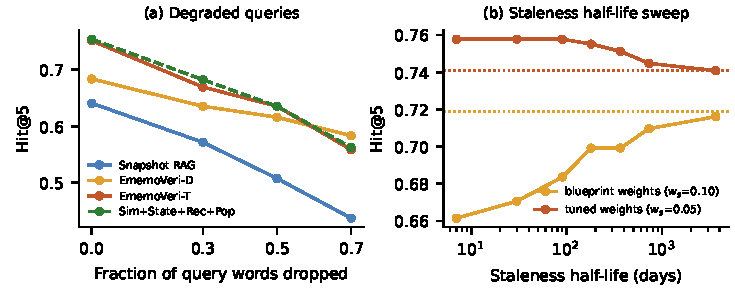
\includegraphics[width=\linewidth]{fig_sweeps.pdf}
\caption{(a) Hit@5 when each query word is dropped with the given probability (weights fixed from dev at 0). (b) Hit@5 against staleness half-life; dotted lines: no staleness term.}
\label{fig:sweeps}
\end{figure}

\textbf{Trust saturates, and a redesign cannot be validated here.} For the top-ranked claim mean trust is \trustMean{} and its AUROC for predicting a correct top-1 answer is \aurocTrustEmv{}, no better than chance (expected calibration error \trustECE{}, which equals one minus accuracy for a constant near 1). The benchmark's evidence is almost all positive (modifications), and the clamped update with $\eta=0.35$ reaches 1 after two or three strong events, so trust cannot separate claims. The non-saturating update does not help ($-$0.007), and trust adds $-$0.003 in the ladder. We did not design a new trust formula: with no negative or independent evidence in this data, a more elaborate model could not be validated, and tuning one to raise the AUROC would be arbitrary.

\textbf{Abstention.} The score gap is informative (AUROC \aurocGapEmv{} default, \aurocGapTuned{} tuned) but a plain similarity gap on snapshot RAG is better (\aurocGapSnap{}). At the prescribed threshold of 0.20 \sys{}-D answers \covTwentyEmv{}\% of tasks (\accTwentyEmv{}\% correct), \sys{}-T \covTwentyTuned{}\% (\accTwentyTuned{}\%) and snapshot RAG \covTwentySnap{}\% (\accTwentySnap{}\%); the coverage--accuracy curves are similar. We find no evidence that the abstention rule adds value over a similarity gap.

\subsection{RQ5: generalisation across repositories and backends}
Results differ by repository: blueprint weights help on fastapi (\repFastEmv{} against \repFastSnap{} for snapshot RAG) and browser-use (\repBuEmv{} against \repBuSnap{}) but hurt on yt-dlp (\repYtdlpEmv{} against \repYtdlpSnap{}); a likely reason, not tested directly, is that yt-dlp has one extractor file per website, so path tokens already match queries well. On fastapi popularity alone reaches \repFastPop{}. Table~\ref{tab:loro} tunes on two repositories and tests on the third. The tuned family beats snapshot retrieval on fastapi (+0.151 [0.076, 0.227]) and browser-use (+0.105 [0.060, 0.150]) but not significantly on yt-dlp (+0.046 [$-$0.015, 0.112]); the tuned design is never significantly different from tuned Sim+Recency+Popularity. The global-tuning yt-dlp figure of \repYtdlpTuned{} includes yt-dlp's own dev period and is therefore optimistic. Hyperparameters in this protocol are tuned on tasks that can postdate the held-out repository's tasks, so it tests transfer across repositories, not causality.

\begin{table}[t]\centering\footnotesize\setlength{\tabcolsep}{3pt}
\resizebox{\linewidth}{!}{\begin{tabular}{lccccll}
\toprule
Held-out ($n$) & Snap. & \sys{}-D & \sys{}-LORO & RP-LORO & LORO$-$Snap. & LORO$-$RP \\
\midrule
fastapi (172) & 0.541 & 0.645 & 0.692 & 0.709 & 0.151 [0.076, 0.227] & $-$0.017 [$-$0.052, 0.017] \\
yt-dlp (196) & 0.801 & 0.689 & 0.847 & 0.832 & 0.046 [$-$0.015, 0.112] & 0.015 [$-$0.005, 0.041] \\
browser-use (400) & 0.605 & 0.698 & 0.710 & 0.710 & 0.105 [0.060, 0.150] & 0.000 [$-$0.018, 0.018] \\
\bottomrule
\end{tabular}}
\caption{Leave-one-repository-out Hit@5 on test-split tasks of the held-out repository (95\% task-bootstrap intervals). \sys{}-LORO: published weight grid tuned on the other two repositories; RP-LORO: Sim+State+Rec+Pop grid tuned likewise.}
\label{tab:loro}
\end{table}

Table~\ref{tab:backends} replaces the hashed TF-IDF similarity by BM25 over the same hashed terms and by cosine of averaged static word vectors (spaCy \texttt{en\_core\_web\_md}; a static embedding, not a neural sentence encoder, which we could not run offline). The priors help with every backend, by +0.057 for BM25 and +0.141 for static vectors, whose lexical ranking is much weaker (0.404). The full prior family is never significantly different from the simple Rec+Pop family, so the conclusion of RQ3 does not depend on the retrieval representation.

\begin{table}[t]\centering\footnotesize\setlength{\tabcolsep}{3pt}
\resizebox{\linewidth}{!}{\begin{tabular}{lcclclc}
\toprule
Backend & Snap. & Full & $\Delta$ vs.\ Snap. & SSRP & $\Delta$ vs.\ Snap. & Full$-$SSRP \\
\midrule
Hashed TF-IDF (main) & 0.641 & 0.741 & 0.100 [0.068, 0.133] & 0.754 & 0.113 [0.082, 0.145] & $-$0.013 [$-$0.031, 0.005] \\
BM25 & 0.641 & 0.698 & 0.057 [0.036, 0.078] & 0.694 & 0.053 [0.033, 0.074] & 0.004 [$-$0.008, 0.016] \\
Static word vectors & 0.404 & 0.544 & 0.141 [0.105, 0.176] & 0.543 & 0.139 [0.107, 0.172] & 0.001 [$-$0.020, 0.022] \\
\bottomrule
\end{tabular}}
\caption{Hit@5 by retrieval backend. Full: frequency, evidence, trust and recency priors; SSRP: Sim+State+Rec+Pop; both tuned on dev for each backend.}
\label{tab:backends}
\end{table}

\subsection{RQ6: vague queries}
\label{sec:degrade}
Commit subjects are more informative than issue text, so we degrade them: each query word is dropped independently with probability 0.3, 0.5 or 0.7 (weights are not re-tuned; this is synthetic noise, not real issue text). Figure~\ref{fig:sweeps}a shows that \sys{}-T keeps a gain over snapshot RAG of +0.098, +0.128 and +0.121 Hit@5 (CIs exclude zero), against +0.111 on the full query; the relative gain grows from 17\% to 28\%. At 0.7 the blueprint weights, which over-weight priors, overtake the tuned weights (0.583 against 0.559). So priors matter at least as much as cues weaken, but the absolute gain is flat rather than growing, and the hypothesis that it increases monotonically is not supported.

\subsection{RQ7: lifecycle events}
\label{sec:life}
We evaluate the state machine directly on events (Table~\ref{tab:life}). For each deletion (395) or rename (38) of a source file after warm-up, the query is the most recent subject touching that file, and we rank before and after the event is ingested. After a deletion naive memory still returns the deleted path in the top five in 33.2\% of cases, while state-aware systems never do. After a rename the new path is in the top five in 76.3\% of cases with history carry-over and 18.4\% without; given that the old path ranked in the top five beforehand, continuity is 96.4\% against 25.0\%. On the twelve held-out repositories (400 deletions, 400 renames) the picture is the same: naive memory returns the deleted path in the top five in 46.3\% of cases and state-aware systems in none; the new path is found in 54.0\% of renames with carry-over and 15.8\% without, and continuity given an earlier hit is 81.9\% against 22.6\%. No superseded claim was revived (0 of 483 at the end of the replay, and 0 on the held-out set), a property the harness guarantees by construction and the regression test of defect~(1) checks inside the engine. Contradiction by revert is rare in the development repositories (16 revert commits touched 22 live claims after warm-up) and more frequent in the held-out set (134 commits, 548 claims), where we count but do not yet score it. API replacement, deprecation, and documentation- or test-versus-code conflicts cannot be recovered from git structure alone, so those paths of the state machine remain unvalidated.

\begin{table}[t]\centering\footnotesize\setlength{\tabcolsep}{3pt}
\resizebox{\linewidth}{!}{\begin{tabular}{lcccc}
\toprule
 & Naive memory & Snapshot RAG & \sys{}-T & Snapshot, no rename carry-over \\
\midrule
Deleted file in top-5 before / after deletion ($n=395$) & 32.2\% / 33.2\% & 32.2\% / 0.0\% & 29.6\% / 0.0\% & -- \\
Old path in top-5 after rename ($n=38$) & 71.1\% & 0.0\% & 0.0\% & -- \\
New path in top-5 after rename & 73.7\% & 76.3\% & 71.1\% & 18.4\% \\
\quad given old path was in top-5 before ($n=28$) & -- & 96.4\% & -- & 25.0\% \\
\bottomrule
\end{tabular}}
\caption{Lifecycle events. Query: latest subject touching the file; top-5 membership of the old or new path before and after the event.}
\label{tab:life}
\end{table}

\subsection{RQ8: confirmation on twelve held-out repositories}
\label{sec:heldout}
The development repositories shaped the code, the baselines and the tuning, so we test the conclusions on twelve others (flask, requests, httpx, rich, black, poetry, pydantic, scrapy, pytest, aiohttp, celery, sphinx; 273--400 tasks each, 4{,}636 in total, pinned heads released). The protocol was written before any of these results were computed (\texttt{docs/PROTOCOL\_V04.md}): systems are frozen with the weights chosen on the original dev split, three directional hypotheses are declared, and inference treats the \emph{repository} as the unit (macro-average, bootstrap over the 12 repositories).

\begin{table}[t]\centering\footnotesize\setlength{\tabcolsep}{3pt}
\resizebox{\linewidth}{!}{\begin{tabular}{lccccc}
\toprule
System (frozen) & Hit@1 & Hit@5 & MRR & NDCG@5 & Dead@5 \\
\midrule
Recency prior & 0.199 & 0.466 & 0.326 & 0.308 & 0.000 \\
Popularity prior & 0.145 & 0.414 & 0.275 & 0.249 & 0.000 \\
Naive memory & 0.286 & 0.518 & 0.395 & 0.376 & 0.349 \\
Snapshot RAG & 0.353 & 0.603 & 0.469 & 0.447 & 0.000 \\
\sys{}-D (blueprint) & 0.365 & 0.636 & 0.488 & 0.467 & 0.000 \\
\sys{}-T (tuned) & 0.401 & 0.693 & 0.531 & 0.516 & 0.000 \\
Sim+State+Rec+Pop & 0.410 & 0.696 & 0.538 & 0.521 & 0.000 \\
\bottomrule
\end{tabular}}
\caption{Frozen systems on the twelve held-out repositories (macro-average over repositories; Dead@5 pooled).}
\label{tab:heldsys}
\end{table}

\begin{table}[t]\centering\footnotesize\setlength{\tabcolsep}{3pt}
\resizebox{\linewidth}{!}{\begin{tabular}{lcccc}
\toprule
Contrast & $\Delta$Hit@5 [95\% CI] & W/L & $\Delta$MRR [95\% CI] & Task-boot.\ CI \\
\midrule
H1: \sys{}-T $-$ Snapshot & 0.090 [0.064, 0.117] & 12/0 & 0.063 [0.046, 0.080] & [0.079, 0.102] \\
H2: \sys{}-T $-$ Sim+State+Rec+Pop & $-$0.004 [$-$0.008, 0.001] & 4/7 & $-$0.006 [$-$0.013, 0.000] & [$-$0.011, 0.004] \\
H3: \sys{}-D $-$ Snapshot & 0.033 [$-$0.006, 0.073] & 7/5 & 0.019 [$-$0.013, 0.050] & [0.017, 0.049] \\
\midrule
Ladder: + state filter & 0.084 [0.050, 0.123] & 11/0 & 0.074 [0.048, 0.103] & [0.072, 0.089] \\
Ladder: + frequency prior & 0.068 [0.033, 0.103] & 11/1 & 0.044 [0.023, 0.067] & [0.055, 0.081] \\
Ladder: + evidence & 0.010 [0.000, 0.020] & 8/4 & 0.008 [0.001, 0.016] & [0.003, 0.015] \\
Ladder: + trust & 0.000 [$-$0.001, 0.000] & 1/3 & 0.000 [$-$0.001, 0.000] & [$-$0.002, 0.001] \\
Ladder: + recency & 0.007 [0.001, 0.012] & 7/4 & 0.005 [0.002, 0.008] & [0.002, 0.012] \\
\bottomrule
\end{tabular}}
\caption{Pre-declared contrasts (H1--H3) and ladder steps over the 12 held-out repositories; CIs from bootstrap over repositories (last column: over tasks). W/L: repositories where the first system is better / worse.}
\label{tab:heldcon}
\end{table}

\textbf{H1 is confirmed.} \sys{}-T beats snapshot retrieval by 0.090 Hit@5 (repository-bootstrap CI [0.064, 0.117]) and wins in all 12 repositories (Table~\ref{tab:heldcon}, Figure~\ref{fig:heldout}). \textbf{H2 is confirmed:} the tuned design is again not better than the tuned similarity+state+recency+popularity baseline ($-$0.004 [$-$0.008, 0.001]; it is better in 4 repositories and worse in 7). \textbf{H3 is confirmed:} blueprint weights give +0.033 [$-$0.006, 0.073] over snapshot retrieval, better in 7 repositories and worse in 5, and \sys{}-T beats them in 11 of 12. The ladder replicates in order: the state filter (+0.084) and the frequency prior (+0.068) dominate, typed evidence adds +0.010 with an interval that just reaches zero, trust adds nothing, and recency adds a small +0.007 [0.001, 0.012], slightly more than on the development repositories. Applying the full R5 weights, which were tuned on the development repositories, is worse than the simpler baseline by 0.010 [$-$0.020, 0.000] (MRR $-$0.012, interval excludes zero), so evidence, trust and recency weights do not transfer as well as the frequency prior.

\begin{figure}[t]\centering
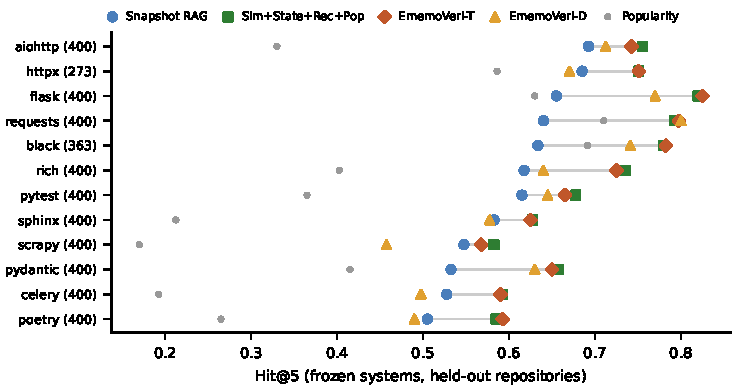
\includegraphics[width=\linewidth]{fig_heldout.pdf}
\caption{Hit@5 per held-out repository (number of tasks in brackets), repositories ordered by snapshot RAG; grey lines join snapshot RAG and \sys{}-T.}
\label{fig:heldout}
\end{figure}

\subsection{Harness validity and robustness}
\label{sec:valid}
The leak canary reaches Hit@1 above \leakSnapOne{}, so a leaking pipeline would be caught. Repeating the main comparison with warm-up 0.20 (839 test tasks), warm-up 0.50 (712) and 150 tasks per repository (315) gives \sys{}-T gains over snapshot RAG of +0.112, +0.088 and +0.111 Hit@5 (all intervals exclude zero), while \sys{}-D is never significantly better after correction and the tuner never gives trust a weight above 0.1.

\section{Discussion}
\textbf{What is supported.} Removing dead files eliminates a real class of error (about 18\% of top-5 slots for naive memory; Dead@5 is 0 for every state-aware system), and carry-over keeps history attached to renamed files. A lexical ranker with a change-frequency prior and a recency prior beats snapshot retrieval by 0.05--0.14 Hit@5 depending on the backend, by 0.09 on average over twelve held-out repositories, under query noise, across resampling schemes and in all twelve held-out repositories.

\textbf{What is not.} The blueprint weights do not reliably beat snapshot retrieval. Over a tuned history prior, \sys{} adds nothing measurable; typed evidence is at best a small refinement of change counts; the trust value carries no signal; and the abstention rule is no better than a similarity gap. For an agent with a working tree the practical recommendation from this benchmark is state-aware similarity plus frequency and recency priors, with weights tuned on the target repository.

\section{Threats to validity}
\label{sec:threats}
\emph{Construct.} File localisation from a commit subject is a proxy for agent tasks and says nothing about patch quality; no real issue or pull-request text is used (building such a set requires authenticated GitHub access that we did not have), so the query degradation in RQ6 is only a stand-in. No language model is in the loop. \emph{Internal.} Tasks are not independent; block and cluster bootstrap widen the intervals but the file-cluster interval for \sys{}-D against snapshot RAG still spans zero by a wide margin. Weights were tuned on the same task family in an earlier period; leave-one-repository-out tuning uses tasks that can postdate the held-out ones. The cumulative ladder is order-dependent. Tie-breaking favours recently updated claims. \emph{External.} Fifteen Python repositories at pinned heads (three for development, twelve held out); only Python source files are tracked and the repositories are popular open-source libraries and tools, so private, multi-language or monorepo settings are untested. \emph{Conclusion.} Holm correction covers the 16 binary comparisons of the original design only; the new intervals are uncorrected.

\section{Audit of the original implementation}
\label{sec:audit}
While building the benchmark we fixed eight defects. (1) SUPERSEDED was not terminal: a later corroboration moved a superseded claim back to CORROBORATED. (2) Retrieval ignored claim state. (3) The temporal leakage guard dropped future evidence but kept the trust and state derived from it; it now replays visible evidence through the trust model and state engine. (4) Staleness defaulted to the wall clock, making every historical claim look fully stale. (5) The keyword relation classifier mislabelled ordinary commits (substring matches on ``add''), so relations now come from git events. (6) Clamped trust updates saturate after two or three strong items. (7) A single candidate always resolved regardless of score. (8) The cross-repository split used object equality in one module and identity in another. Each fix has a regression test; results from before the fixes, including the original synthetic experiments, should not be reused.

\section{Conclusion}
On real repository history, the parts of memory that pay off are state awareness and cheap activity priors: removing dead files, a change-frequency prior and a recency prior account for the measurable gain over similarity retrieval, and a tuned ranker of exactly those ingredients matches dev-tuned \sys{}. Typed evidence is at most a small refinement, trust is uninformative and the abstention rule does not beat a similarity gap, in this evidence regime. The held-out repositories show that these conclusions are not an artefact of the three development repositories. The immediate next steps are queries from real issues and pull requests, a coding agent in the loop on a modest task set to test whether better localisation improves patches, a neural dense retriever, a dedicated contradiction set with negative and independent evidence, and a trust model validated on it.

\paragraph{Reproducibility.} Code, tests, per-task outcomes, summaries and pinned repository heads are in the accompanying repository. \texttt{scripts/}\allowbreak\texttt{reproduce\_real.sh} regenerates the original numbers; \texttt{experiments/}\allowbreak\texttt{collect\_ext.py} and \texttt{experiments/}\allowbreak\texttt{analyze\_ext.py} and \texttt{analyze\_heldout.py} regenerate the new analyses, and \texttt{paper/}\allowbreak\texttt{make\_ext.py} and \texttt{make\_heldout.py} the new tables and figures.

\paragraph{Acknowledgments.} Parts of the benchmark code and of the manuscript text were prepared with a large language model. The author reviewed the output, ran all experiments, and takes full responsibility for the content.

\bibliographystyle{splncs04}
\bibliography{refs}
\end{document}
